\hypertarget{_drift_shell_8c}{
\section{/home/mgh/LanlGeoMag/libLanlGeoMag/DriftShell.c File Reference}
\label{_drift_shell_8c}\index{/home/mgh/LanlGeoMag/libLanlGeoMag/DriftShell.c@{/home/mgh/LanlGeoMag/libLanlGeoMag/DriftShell.c}}
}
{\tt \#include \char`\"{}Lgm/Lgm\_\-MagModelInfo.h\char`\"{}}\par
{\tt \#include \char`\"{}Lgm/Lgm\_\-LstarInfo.h\char`\"{}}\par


Include dependency graph for DriftShell.c:\nopagebreak
\begin{figure}[H]
\begin{center}
\leavevmode
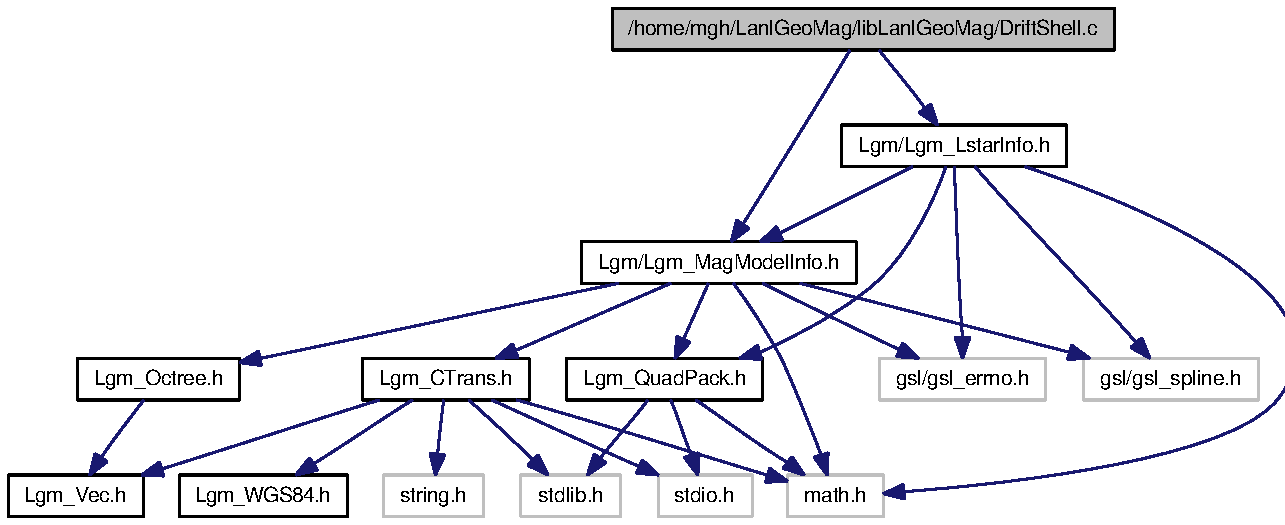
\includegraphics[width=326pt]{_drift_shell_8c__incl}
\end{center}
\end{figure}
\subsection*{Functions}
\begin{CompactItemize}
\item 
int \hyperlink{_drift_shell_8c_e79603e88bcb7860ca33e8fe4fbdf37f}{FindShellLine} (double I0, double $\ast$Ifound, double Bm, double MLT, double $\ast$mlat, double $\ast$rad, double mlat0, double mlat1, \hyperlink{struct_lgm___lstar_info}{Lgm\_\-LstarInfo} $\ast$LstarInfo)
\item 
int \hyperlink{_drift_shell_8c_15d887d6b99cb83ce58b5a04a171ec67}{FindBmRadius} (double Bm, double MLT, double mlat, double $\ast$r, double tol, \hyperlink{struct_lgm___lstar_info}{Lgm\_\-LstarInfo} $\ast$LstarInfo)
\end{CompactItemize}


\subsection{Function Documentation}
\hypertarget{_drift_shell_8c_e79603e88bcb7860ca33e8fe4fbdf37f}{
\index{DriftShell.c@{DriftShell.c}!FindShellLine@{FindShellLine}}
\index{FindShellLine@{FindShellLine}!DriftShell.c@{DriftShell.c}}
\subsubsection[{FindShellLine}]{\setlength{\rightskip}{0pt plus 5cm}int FindShellLine (double {\em I0}, \/  double $\ast$ {\em Ifound}, \/  double {\em Bm}, \/  double {\em MLT}, \/  double $\ast$ {\em mlat}, \/  double $\ast$ {\em rad}, \/  double {\em mlat0}, \/  double {\em mlat1}, \/  {\bf Lgm\_\-LstarInfo} $\ast$ {\em LstarInfo})}}
\label{_drift_shell_8c_e79603e88bcb7860ca33e8fe4fbdf37f}




Definition at line 36 of file DriftShell.c.

Here is the call graph for this function:\nopagebreak
\begin{figure}[H]
\begin{center}
\leavevmode
\includegraphics[width=401pt]{_drift_shell_8c_e79603e88bcb7860ca33e8fe4fbdf37f_cgraph}
\end{center}
\end{figure}


Here is the caller graph for this function:\nopagebreak
\begin{figure}[H]
\begin{center}
\leavevmode
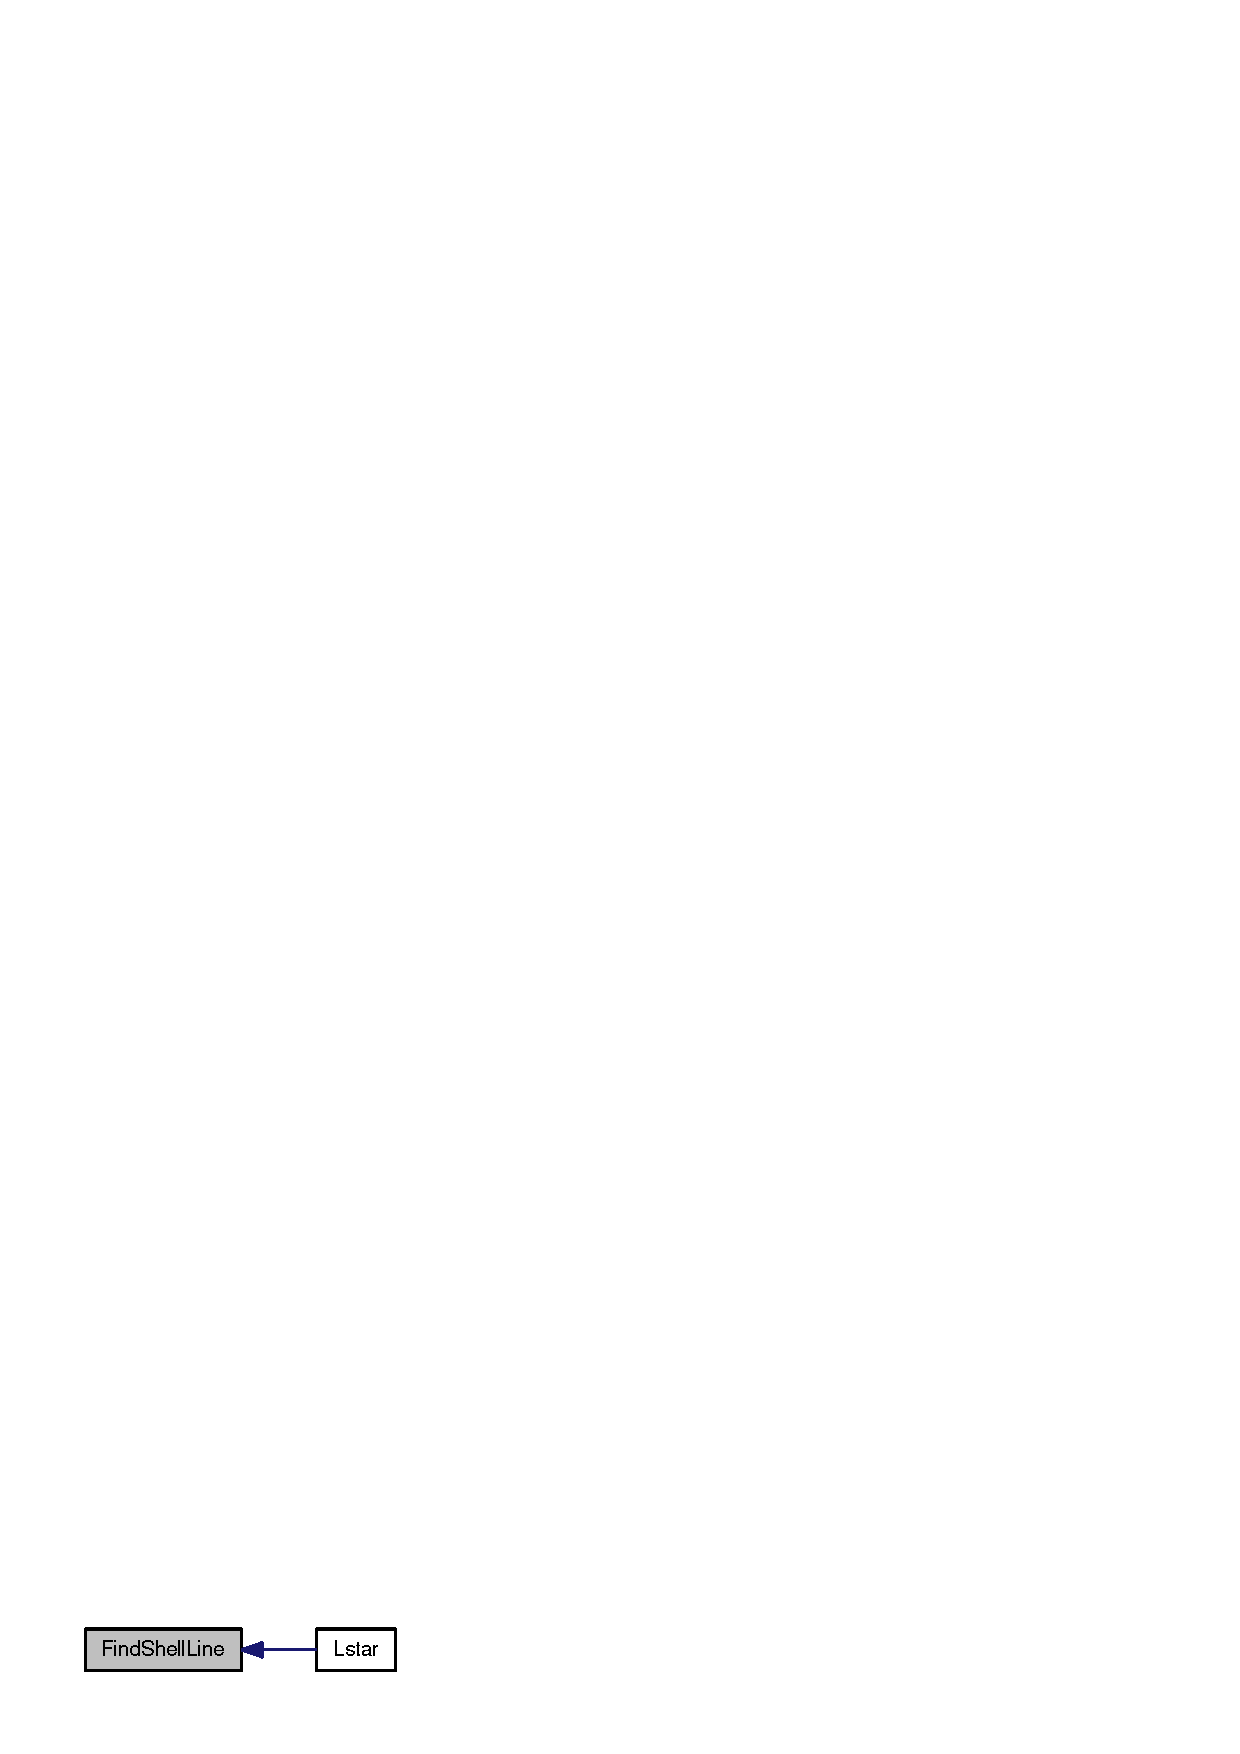
\includegraphics[width=97pt]{_drift_shell_8c_e79603e88bcb7860ca33e8fe4fbdf37f_icgraph}
\end{center}
\end{figure}
\hypertarget{_drift_shell_8c_15d887d6b99cb83ce58b5a04a171ec67}{
\index{DriftShell.c@{DriftShell.c}!FindBmRadius@{FindBmRadius}}
\index{FindBmRadius@{FindBmRadius}!DriftShell.c@{DriftShell.c}}
\subsubsection[{FindBmRadius}]{\setlength{\rightskip}{0pt plus 5cm}int FindBmRadius (double {\em Bm}, \/  double {\em MLT}, \/  double {\em mlat}, \/  double $\ast$ {\em r}, \/  double {\em tol}, \/  {\bf Lgm\_\-LstarInfo} $\ast$ {\em LstarInfo})}}
\label{_drift_shell_8c_15d887d6b99cb83ce58b5a04a171ec67}




Definition at line 344 of file DriftShell.c.

Here is the call graph for this function:\nopagebreak
\begin{figure}[H]
\begin{center}
\leavevmode
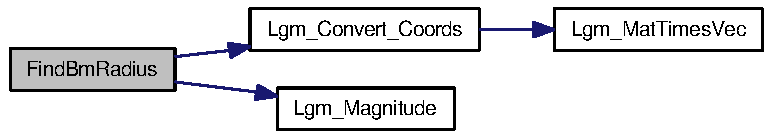
\includegraphics[width=203pt]{_drift_shell_8c_15d887d6b99cb83ce58b5a04a171ec67_cgraph}
\end{center}
\end{figure}


Here is the caller graph for this function:\nopagebreak
\begin{figure}[H]
\begin{center}
\leavevmode
\includegraphics[width=155pt]{_drift_shell_8c_15d887d6b99cb83ce58b5a04a171ec67_icgraph}
\end{center}
\end{figure}
